\begin{figure*}[t!]
    \centering
    
\includegraphics[width=0.95\linewidth]{figures/overview.pdf}
    \caption{Overview of \model. We illustrate the workflow across three consecutive training steps; for simplicity, we only show the speculative decoding process for step $N$.}
    \label{fig:overview}
\end{figure*}

\section{\model Design} 


\model provides a systematic, lossless rollout-phase optimization that leverages idle bubbles to efficiently pre-generate draft responses and thereby enable fast speculative decoding, while remaining a modular component that can be seamlessly integrated into various synchronous RL frameworks. In \autoref{sec:3_1}, we describe how \model schedules rollout pre-generation into these idle bubbles; we then show how the resulting partial rollouts are used for efficient speculative decoding with low draft overhead (\autoref{sec:3_2}) and verification overhead (\autoref{sec:3_3}), ensuring that the reduction in decoding steps translates directly into a reduction in rollout time.

\subsection{Use GPU Bubbles for Rollout Pre-Generation}
\label{sec:3_1}

As mentioned, our key objective is to harvest idle compute for draft pre-generation while avoiding interference with the main rollout and keeping synchronization overhead low.

\textbf{Inter-GPU Bubbles vs. Intra-GPU Bubbles.}
We first consider how to utilize bubbles without disrupting current batch generation, and in particular, whether to exploit inter-GPU or intra-GPU bubbles. 
Intra-GPU bubbles can expose more time for pre-generation, but they directly contend with the running decoding workload. 
We experiment with a selective intra-GPU strategy: among all DP ranks, we use only the intra-GPU bubbles of the fastest ranks (\eg 6 out of 8) once their effective batch size drops below a threshold. We observed highly unstable interference: Fast ranks are slowed down after taking additional requests and may even finish later than the original stragglers. 
Instead, we found inter-GPU bubbles alone are sufficient to generate enough draft tokens while avoiding extra contention and instability. 
Therefore, we exploit only the inter-GPU bubbles for rollout pre-generation.


\textbf{Rollout DP Rank Synchronization.}
Another key design choice is how to synchronize rollout DP ranks so that pre-generation can stop once the slowest rank finishes the current batch. Since per-step decoding lasts for only a few milliseconds, naive cross-GPU or cross-node synchronization can incur disproportionate overhead. 
We therefore adopt a periodic polling scheme: during the pre-generation of \(B_{t+1}\), each rank queries a central synchronizer every \(T\) decoding steps. If the synchronizer reports that all ranks have completed \(B_t\), pre-generation is halted, and the system proceeds to the barrier. 
The parameter \(T\) is tuned to balance the freshness of synchronization against the cost of inter-process communication, keeping coordination overhead negligible compared to decoding.

\textbf{Pre-Generation Batch Size.}
Finally, we decide how many samples to pre-generate per prompt. A larger pre-generation batch size explores more decoding paths for a single prompt, increasing diversity and the probability of prefix matches during speculative decoding. However, an excessively large batch size also increases per-step decoding latency, which can reduce the maximum response length that can be served and may leave prompts with long responses under-covered at later positions. 
We empirically match the number of pre-generated samples per prompt with the number of samples used in GRPO for each prompt group, and find that this choice well balances the diversity and coverage.


\subsection{Suffix Tree-based Speculative Decoding}
\label{sec:3_2}
To exploit pre-generated partial rollouts as speculative drafts, the system should repetitively match the current rollout prefix against a large pool of historical tokens and retrieve likely continuations with minimal online overhead, \ie draft overhead. 
This requirement naturally leads to a design that separates \textit{offline indexing} from \textit{online lookup}.

We consider two generic indexing strategies for prefix matching over historical rollouts: 1) an \emph{n-gram–style} scheme that performs pattern matching directly over raw token sequences, and 2) a \emph{suffix-based} scheme that builds an explicit index over all suffixes. 
The former requires no explicit index, but its per-query cost is proportional to the history length, which can be prohibitive over thousands of decoding steps. 
The latter amortizes work by building a compact suffix index over the pre-generated tokens, so that lookup depends primarily on the prefix length and the number of matches, and is effectively decoupled from the total history size.

Since speculative decoding issues a large number of prefix-matching queries during rollout, we adopt the \textbf{suffix-based design}. 
Conceptually, the system aggregates pre-generated rollouts into prompt-associated token pools and constructs a suffix index for each pool. 
The indices are sharded across rollout workers following the existing rollout dispatch: each rollout DP rank builds and maintains suffix indices only for the prompts it is responsible for generating. 
As a result, the construction cost depends on the local prompt set instead of the global training scale, and the indexing layer scales with system size without a centralized bottleneck. This parallelization bounds the suffix tree construction overhead as the system scales up.

%%%%%%%%%%%%%%%%%%%%%
\yuhang{At each decoding step, we retrieve a block of candidate tokens conditioned on the current prefix, which provides a deterministic proposal for model-free speculative decoding. Concretely, let $\tilde{x}_t$ denote the retrieved draft token at step $t$, and let $p_t(\cdot)$ be the \emph{actual} decoding distribution used by the target policy at that step, after temperature scaling and any top-$p$/top-$k$ filtering. We accept $\tilde{x}_t$ with probability
\begin{equation}
    P_{\mathrm{accept}} = p_t(\tilde{x}_t).
\end{equation}

Equivalently, this is rejection sampling with a degenerate proposal $q_t(\tilde{x}_t)=1$. If the draft token is rejected, we sample a recovered token from the residual distribution
\begin{equation}
    r_t(x)=\frac{p_t(x)\mathbf{1}[x\neq \tilde{x}_t]}{1-p_t(\tilde{x}_t)}.
\end{equation}
In the multi-token case, we verify a retrieved draft block sequentially and accept tokens until the first rejection; upon rejection, we draw one recovered token from the corresponding residual distribution and restart drafting from the updated prefix. If all draft tokens are accepted, we continue decoding from the extended prefix. Therefore, BubbleSpec exactly preserves the target rollout distribution while reducing the number of decoding steps. Compared with history-based methods that rely on cross-epoch policy similarity, our acceptance behavior depends on the quality of the suffix-tree proposal under the current policy, while the correctness guarantee follows directly from the rejection-sampling construction. A full pseudocode of the speculative decoding procedure is provided in Appendix~\ref{sec:spec_details}.}

\begin{figure}[t!]
    \centering
    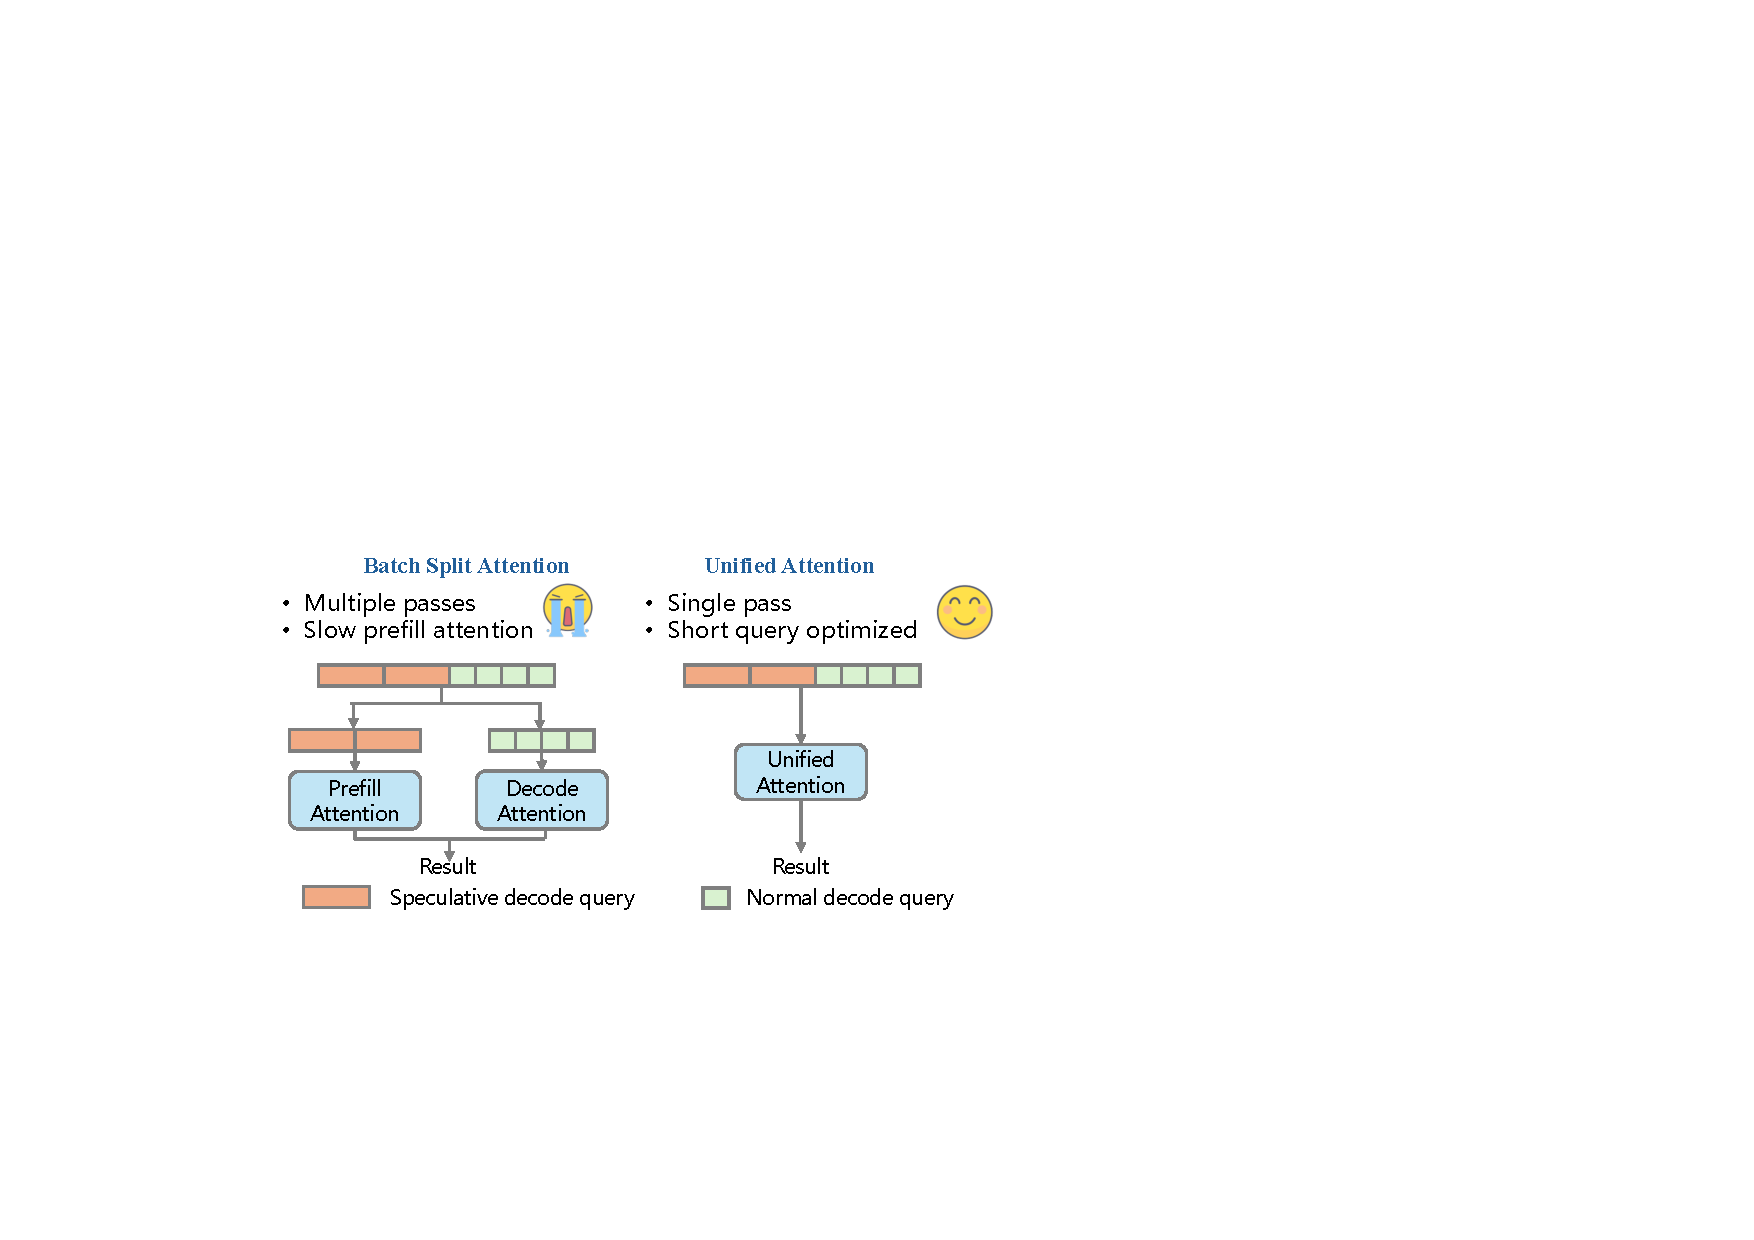
\includegraphics[width=1\linewidth]{figures/unified_attn.pdf}
    \caption{Comparison between batch split and unified attention.}
    \label{fig:unified_attn}
\end{figure}

% Please add the following required packages to your document preamble:
% \usepackage{booktabs}
% \usepackage{graphicx}
\begin{table}[t!]
\centering
\caption{Latency of attention operators in speculative decoding.}
\label{tab:attn_latency}
\resizebox{\linewidth}{!}{%
\begin{tabular}{@{}clccc@{}}
\toprule
\multicolumn{2}{c}{\multirow{2}{*}{\textbf{\begin{tabular}[c]{@{}c@{}}Normal Attention w/o.\\ Speculative Queries\end{tabular}}}} & \multicolumn{2}{c}{\textbf{Batch Split Attention}} & \multirow{2}{*}{\textbf{Unified Attention}} \\ \cmidrule(lr){3-4}
\multicolumn{2}{c}{} & \textbf{Prefill} & \textbf{Decode} &  \\ \midrule
\multicolumn{2}{c}{0.372 ms} & 0.753 ms & 0.226 ms & 0.380 ms \\ \bottomrule
\end{tabular}%
}
\end{table}

\subsection{Unified Attention for Speculative Decoding}
\label{sec:3_3}
% As analyzed in \autoref{sec:spec_decoding}, while suffix decoding reduces decoding steps with neglible draft overheads, its real acceleration effect is still constrained by increased draft overhead. In practice, we found that even the number of draft tokens is limited, without much computation increasement, \ie the system is still memory-bounded, we still oberserve substantial per-step decoding latency increase, largely offsetting the advantage of less steps. 

% While previous works simply attribute this inefficiency to larger computation casued by larger batch size, we found that a large part of this inefficiency is due to inefficient batching behaviour with draft tokens. Specifically, the operations in LLM forward pass can be categorized into two: (1) \textbf{token-wise} operation such as linear, layernorm can be efficiently batched regardless of the request length. (2) \textbf{request-wise} operation, typically, attention, exhibit complex performance behaviour under different request batching strategies. Specifically, the introduce of draft tokens make the query length of attention may be larger than 1, the same scenario as prefill attention which also have query length larger than 1. Existing inference engine adopt different operations for prefill and decode attention due to the their distinct resource utilization characteriscs. When meeting draft tokens in speculative decoding, they will adopt the inefficient prefill attention for the request with draft tokens.  

As analyzed in \autoref{sec:spec_decoding}, although suffix decoding reduces decoding steps with low draft overhead, its actual acceleration is constrained by increased per-step latency due to the verification overhead. 
We find that even when the number of draft tokens is limited (\ie introducing little extra computation and keeping the system memory-bound), there is still a substantial increase in per-step decoding latency, offsetting the benefit of fewer steps. 
% 
While prior work typically attributes this inefficiency to the increased computation from larger batch sizes, we identify that it is mainly caused by \textit{suboptimal batching behavior with draft tokens}. 

Operations in the LLM forward pass can be divided into: (1) \textbf{Token-wise} operations, such as linear layers and layer normalization, which can be efficiently batched regardless of request length; and (2) \textbf{Request-wise} operations, primarily attention, whose performance is highly sensitive to batching strategies. 
The draft tokens make the attention query length greater than 1, similar to prefill attention. Existing inference engines use different kernels for prefill and decode attention due to their distinct resource characteristics. 
When draft tokens appear in speculative decoding, they trigger the less efficient prefill-style attention. As shown in \autoref{fig:unified_attn}, this split-attention behavior partitions the batch into two groups: requests with draft tokens use prefill attention, and other requests use standard decode attention.

We show this inefficiency in \autoref{tab:attn_latency}. The experiment is conducted with batch size 128 and context length 8k, where 32 requests are speculative with 4 draft tokens each. 
Although the total number of tokens increases only from 128 to 256, the latency under batch-split attention is nearly three times that of normal attention without draft tokens, primarily due to the prefill attention. 

To address these issues, we optimize the attention implementation within the rollout engine by adopting a unified attention operator capable of handling variable query lengths within a short range, as shown in \autoref{fig:unified_attn}. 
This unified operator processes normal and decode queries within a single CUDA kernel launch, eliminating batch splitting overhead. 
The matrix multiplications for short-query verification are efficiently executed on tensor cores~\cite{markidis2018nvidia_tensor} in modern GPUs, whose fixed tile sizes ensure negligible latency increase as long as the problem size remains small. 
As shown in \autoref{tab:attn_latency}, unified attention incurs almost no additional latency for speculative requests compared to normal attention without speculative queries, ensuring that the reduced number of decoding steps translates into real end-to-end generation speedup. 
